% !TeX program = xelatex
% Standalone source. Compile with XeLaTeX; no external figures are required.
\documentclass[11pt,a4paper]{article}
\usepackage[margin=20mm]{geometry}
\usepackage{fontspec}
\usepackage{xeCJK}
\IfFontExistsTF{Times New Roman}{\setmainfont{Times New Roman}}{\setmainfont{Latin Modern Roman}}
\IfFontExistsTF{Microsoft JhengHei}{\setCJKmainfont{Microsoft JhengHei}}{
  \IfFontExistsTF{Noto Serif CJK TC}{\setCJKmainfont{Noto Serif CJK TC}}{\setCJKmainfont{FandolSong-Regular}}}
\IfFontExistsTF{Microsoft JhengHei}{\setCJKmonofont{Microsoft JhengHei}}{
  \IfFontExistsTF{Noto Serif CJK TC}{\setCJKmonofont{Noto Serif CJK TC}}{\setCJKmonofont{FandolSong-Regular}}}
\usepackage{amsmath,amssymb,booktabs,array,xcolor,tikz,fancyhdr,hyperref}
\usetikzlibrary{calc,arrows.meta}
\hypersetup{colorlinks=true,linkcolor=blue!50!black,urlcolor=blue!50!black}
\definecolor{accent}{HTML}{124E66}
\definecolor{pcol}{HTML}{A24021}
\definecolor{ncol}{HTML}{175A86}
\pagestyle{fancy}\fancyhf{}\fancyhead[L]{\small EE3032 / Fall 2024 / HW1}
\fancyhead[R]{\small CMOS logic}\fancyfoot[C]{\thepage}
\setlength{\headheight}{15pt}\setlength{\parindent}{0pt}\setlength{\parskip}{6pt}
\renewcommand{\arraystretch}{1.2}
\newcommand{\answer}[1]{\par\noindent\colorbox{accent!9}{\parbox{0.96\linewidth}{#1}}\par}
\newcommand{\AND}{\,}
\newcommand{\VDD}{V_{\mathrm{DD}}}
\newcommand{\VSS}{V_{\mathrm{SS}}}
% A conventional switch-level MOS symbol: continuous channel, insulated gate,
% and a gate bubble for pMOS. Bulk terminals are omitted, as explained below.
% Arguments: device id, x, y, gate literal, p or n. t/b are upper/lower terminals.
\newcommand{\MOS}[5]{
  \coordinate (#1) at (#2,#3);
  \coordinate (#1t) at ($(#1)+(0,.55)$);
  \coordinate (#1b) at ($(#1)+(0,-.55)$);
  \draw (#1t)--($(#1)+(0,.30)$)--($(#1)+(-.18,.30)$);
  \draw ($(#1)+(-.18,.34)$)--($(#1)+(-.18,-.34)$);
  \draw ($(#1)+(-.18,-.30)$)--($(#1)+(0,-.30)$)--(#1b);
  \draw ($(#1)+(-.35,.33)$)--($(#1)+(-.35,-.33)$);
  \def\type{#5}\def\ptype{p}
  \ifx\type\ptype
    \draw ($(#1)+(-.78,0)$)--($(#1)+(-.53,0)$);
    \draw ($(#1)+(-.465,0)$) circle (.065);
    \draw ($(#1)+(-.40,0)$)--($(#1)+(-.35,0)$);
  \else
    \draw ($(#1)+(-.78,0)$)--($(#1)+(-.35,0)$);
  \fi
  \node[anchor=east] at ($(#1)+(-.82,0)$) {$#4$};
  \node[anchor=west,font=\scriptsize] at ($(#1)+(.10,0)$) {#1};
}
% A transmission-gate instance; its two MOS devices are expanded on page 3.
\newcommand{\TG}[4]{
  \node[draw,rounded corners=1pt,minimum width=11mm,minimum height=6mm,
        fill=accent!5,font=\small] (#1) at (#2,#3) {$\mathrm{TG}_{#4}$};
}
\begin{document}
\begin{center}
{\LARGE\bfseries 2024 Homework 1}\\[4pt]
{\large Static CMOS、資料選擇電路與 XNOR}\\[4pt]
{\small Introduction to VLSI Design / Jin-Fu Li / EE3032}
\end{center}
\textbf{解題與符號。}本解答先依原題推導，再比對資料夾中的兩份手寫答案。
式中的 $+$ 為 OR、相乘為 AND、上橫線為 NOT。所有電晶體圖省略 body：
pMOS body 接 $\VDD$，nMOS body 接 $\VSS=0$。pMOS gate 的小圓圈表示低電位導通。
題 1 只提供正相輸入；本解答的題 1 不需要額外反相器。

\section*{1(a) 吸收律後為二輸入 NOR}
\textbf{原題讀式：}反相橫線涵蓋整個 $x+y+w y z$，因此
\begin{align*}
 f(w,x,y,z)&=\overline{x+y+w y z}\\
 &=\overline{x+y(1+wz)}=\boxed{\overline{x+y}}.
\end{align*}
因為 $y+w y z=y$，輸出與 $w,z$ 無關。下拉網路（PDN）用 $x,y$ 兩顆 nMOS
並聯；上拉網路（PUN）是其對偶，兩顆 pMOS 串聯。
\begin{center}
\begin{tikzpicture}[x=1cm,y=.68cm,line width=.8pt,font=\small]
 \MOS{P1}{0}{6.7}{x}{p}\MOS{P2}{0}{5.2}{y}{p}
 \MOS{N1}{-1}{2.1}{x}{n}\MOS{N2}{1.6}{2.1}{y}{n}
 \draw (-1,7.7)--(1.6,7.7) node[right] {$\VDD$};
 \draw (0,7.7)--(P1t) (P1b)--(P2t) (P2b)--(0,3.6);
 \draw (-1,3.6)--(2.6,3.6) node[right] {$f$};
 \draw (-1,3.6)--(N1t) (1.6,3.6)--(N2t);
 \draw (N1b)--(-1,.8)--(1.6,.8)--(N2b);
 \node[below] at (.3,.8) {$\VSS$};
 \fill (0,3.6) circle (1.7pt) (1.6,3.6) circle (1.7pt);
 \node[anchor=west,text=pcol] at (3,6) {PUN：$\bar x\bar y$};
 \node[anchor=west,text=ncol] at (3,2.1) {PDN：$x+y$};
\end{tikzpicture}
\end{center}
\begin{center}
\begin{tabular}{ccccc}\toprule
$x$&$y$&$w,z$&PDN 導通&$f$\\\midrule
0&0&任意&0&1\\0&1&任意&1&0\\1&0&任意&1&0\\1&1&任意&1&0\\\bottomrule
\end{tabular}
\end{center}
\answer{\textbf{採用 4T NOR。}直接照未化簡式畫圖需 5 顆 nMOS 與 5 顆 pMOS，
但其中 $wyz$ 支路不改變邏輯。保留它可實現原式；刪除後可省 6 顆電晶體。}

\newpage
\section*{1(b) 三輸入 minority function：10T static CMOS}
原題為 $f=\bar x\bar y+\bar x\bar z+\bar y\bar z$。
先把輸出反相，便能以正相輸入實作 nMOS PDN：
\begin{align*}
 \bar f&=(x+y)(x+z)(y+z)=xy+xz+yz\\
 &=xy+z(x+y),\\
 f&=\overline{xy+z(x+y)}
   =(\bar x+\bar y)(\bar z+\bar x\bar y).
\end{align*}
PDN 左支路為 $x$ 串 $y$，右支路為 $z$ 串 $(x\parallel y)$。
PUN 為 $(x\parallel y)$ 串 $[z\parallel(x\text{ 串 }y)]$，gate 均接正相輸入。
\begin{center}
\begin{tikzpicture}[x=.83cm,y=.52cm,line width=.8pt,font=\small]
 \MOS{P1}{0}{10.7}{x}{p}\MOS{P2}{3.2}{10.7}{y}{p}
 \MOS{P3}{0}{7.3}{z}{p}\MOS{P4}{3.2}{8.15}{x}{p}\MOS{P5}{3.2}{6.45}{y}{p}
 \draw (-.5,12)--(3.7,12) node[right] {$\VDD$};
 \draw (0,12)--(P1t) (3.2,12)--(P2t);
 \draw (P1b)--(0,9.4)--(3.2,9.4)--(P2b);
 \draw (0,9.4)--(P3t) (3.2,9.4)--(P4t) (P4b)--(P5t);
 \draw (P3b)--(0,5.1)--(3.2,5.1)--(P5b);
 \draw (3.2,5.1)--(4.7,5.1) node[right] {$f$};
 \MOS{N1}{0}{3.7}{x}{n}\MOS{N2}{0}{1.6}{y}{n}
 \MOS{N3}{3.2}{3.7}{z}{n}\MOS{N4}{2}{1.6}{x}{n}\MOS{N5}{4.4}{1.6}{y}{n}
 \draw (0,5.1)--(N1t) (N1b)--(N2t);
 \draw (3.2,5.1)--(N3t) (N3b)--(3.2,2.6);
 \draw (2,2.6)--(4.4,2.6) (2,2.6)--(N4t) (4.4,2.6)--(N5t);
 \draw (N2b)--(0,.3)--(4.4,.3)--(N5b) (N4b)--(2,.3);
 \node[below] at (2,.3) {$\VSS$};
 \foreach \x/\y in {0/9.4,3.2/9.4,0/5.1,3.2/5.1,3.2/2.6,2/.3}
   \fill (\x,\y) circle (1.6pt);
 \node[anchor=west,text=pcol] at (6,9) {PUN：5 顆 pMOS};
 \node[anchor=west,text=ncol] at (6,2.6) {PDN：5 顆 nMOS};
\end{tikzpicture}
\end{center}
\begin{center}
\begin{tabular}{cccccc}\toprule
$x$&$y$&$z$&$xy+z(x+y)$&$f$&PUN 導通\\\midrule
0&0&0&0&1&1\\0&0&1&0&1&1\\0&1&0&0&1&1\\0&1&1&1&0&0\\
1&0&0&0&1&1\\1&0&1&1&0&0\\1&1&0&1&0&0\\1&1&1&1&0&0\\\bottomrule
\end{tabular}
\end{center}
\answer{\textbf{共 10T，無輸入反相器。}恰有至多一個輸入為 1 時輸出為 1。
兩份手寫答案的 12T 結構也正確；此處用因式分解省下 2T。}

\newpage
\section*{2. 四路循環資料選擇：CMOS transmission gates}
表中每列恰有一個 $c_j=1$，以下以此 \textbf{one-hot} 條件設計。
每個輸出用四個 transmission gate（TG）選一個資料輸入：
\begin{align*}
z_3&=c_3a_3+c_2a_2+c_1a_1+c_0a_0,\\
z_2&=c_3a_2+c_2a_1+c_1a_0+c_0a_3,\\
z_1&=c_3a_1+c_2a_0+c_1a_3+c_0a_2,\\
z_0&=c_3a_0+c_2a_3+c_1a_2+c_0a_1.
\end{align*}
等價的接線索引為 $z_i\leftarrow a_{(i+j-3)\bmod4}$，其中 $c_j=1$。
下頁完整列出 16 個 TG 的資料接線，並共用四組 $c_j,\bar c_j$。

\subsection*{TG 的電晶體展開與互補控制}
\begin{center}
\begin{tikzpicture}[x=.85cm,y=.65cm,line width=.8pt,font=\small]
 \MOS{Nj}{0}{2.5}{c_j}{n}\MOS{Pj}{3.6}{2.5}{\bar c_j}{p}
 \draw (Njt)--(0,4)--(3.6,4)--(Pjt);
 \draw (Njb)--(0,1)--(3.6,1)--(Pjb);
 \draw (0,4)--(-1.7,4) node[left] {$d$};
 \draw (3.6,1)--(5.1,1) node[right] {$q$};
 \node[anchor=west] at (5.7,3) {$c_j=1$: nMOS、pMOS 都導通};
 \node[anchor=west] at (5.7,2) {$c_j=0$: nMOS、pMOS 都截止};
\end{tikzpicture}
\end{center}
圖中兩顆 MOS \textbf{並聯於相同的資料端點}。與 NMOS-only pass gate 相比，
TG 能傳遞完整的高、低邏輯電位。因為資料可雙向通過，圖中的上下端點是資料端，
並非接電源；body 仍分別接 $\VSS$ 與 $\VDD$。

\subsection*{共用反相器（四份，$j=0,1,2,3$）}
\begin{center}
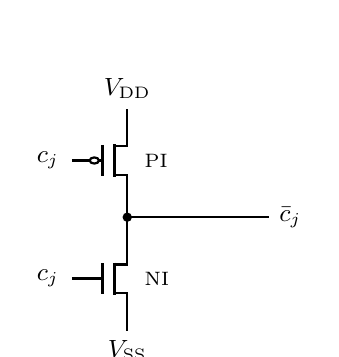
\begin{tikzpicture}[x=.9cm,y=.6cm,line width=.8pt,font=\small]
 \MOS{PI}{0}{4.7}{c_j}{p}\MOS{NI}{0}{2.2}{c_j}{n}
 \draw (PIt)--(0,5.8) node[above] {$\VDD$};
 \draw (PIb)--(0,3.5)--(NIt);
 \draw (0,3.5)--(2,3.5) node[right] {$\bar c_j$};
 \draw (NIb)--(0,1.1) node[below] {$\VSS$};
 \fill (0,3.5) circle (1.7pt);
\end{tikzpicture}
\end{center}
\answer{\textbf{電晶體數：}$16\text{ TG}\times2+4\text{ inverter}\times2=40\text{T}$。
不含非題目要求的輸出 buffer。只有 one-hot 的四列被指定；零選擇時輸出浮接，
多個選擇時可能把不同資料短接，因此控制器必須維持 one-hot 並避免重疊切換。}

\newpage
\section*{2. 完整 TG 接線圖與表格驗證（續）}
每個 $\mathrm{TG}_j$ 是上頁的兩顆 MOS，nMOS gate 接 $c_j$，pMOS gate 接 $\bar c_j$。
四個圖中的同名控制線由同一組反相器供應；不同輸出之間沒有資料接點。
\begin{center}
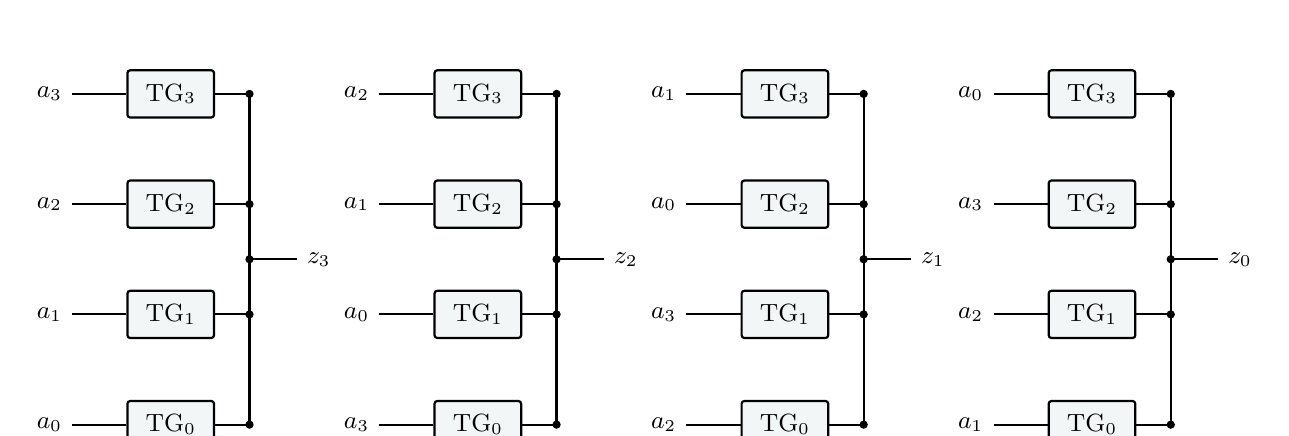
\begin{tikzpicture}[x=1cm,y=1cm,line width=.8pt,font=\small]
 \foreach \col/\zi in {0/3,1/2,2/1,3/0}{
   \begin{scope}[xshift=\col*3.9cm]
   \foreach \row/\cj in {0/3,1/2,2/1,3/0}{
     \pgfmathtruncatemacro{\ai}{mod(\zi+\cj+1,4)}
     \TG{tg\zi\cj}{1.25}{-\row*1.4}{\cj}
     \draw (0,-\row*1.4) node[left] {$a_{\ai}$}--(tg\zi\cj.west);
     \draw (tg\zi\cj.east)--(2.25,-\row*1.4);
     \fill (2.25,-\row*1.4) circle (1.5pt);
   }
   \draw (2.25,0)--(2.25,-4.2);
   \draw (2.25,-2.1)--(2.85,-2.1) node[right] {$z_{\zi}$};
   \fill (2.25,-2.1) circle (1.5pt);
   \end{scope}
 }
\end{tikzpicture}
\end{center}
\vspace{8pt}
\begin{center}
\begin{tabular}{ccccccccc}\toprule
$c_3$&$c_2$&$c_1$&$c_0$&導通 TG&$z_3$&$z_2$&$z_1$&$z_0$\\\midrule
1&0&0&0&所有 $\mathrm{TG}_3$&$a_3$&$a_2$&$a_1$&$a_0$\\
0&1&0&0&所有 $\mathrm{TG}_2$&$a_2$&$a_1$&$a_0$&$a_3$\\
0&0&1&0&所有 $\mathrm{TG}_1$&$a_1$&$a_0$&$a_3$&$a_2$\\
0&0&0&1&所有 $\mathrm{TG}_0$&$a_0$&$a_3$&$a_2$&$a_1$\\\bottomrule
\end{tabular}
\end{center}
\textbf{一列的檢查範例。}令 $c_2=1$，其餘為 0。則每個輸出只有
$\mathrm{TG}_2$ 導通，沿接線可直接得到
\[
 (z_3,z_2,z_1,z_0)=(a_2,a_1,a_0,a_3).
\]
其餘三列同理。附帶的 Python 驗證對四個 one-hot 選擇與全部 16 組資料逐一檢查，
共 $4\times16=64$ 組；除了方程式，亦檢查展開為 nMOS/pMOS 後的連通性。

\subsection*{若需要所有控制碼都有定義}
原表未指定的 12 組控制碼不應自行視為 one-hot TG 的有效操作。
若規格改為任意 $c_0,\ldots,c_3$ 都必須實現上述 AND-OR 方程式，可對每個
$z_i$ 用四個 NAND2 產生 $\overline{c_j a_k}$，再用 NAND4 合併；每輸出
$4\times4+8=24$T，共 96T。此方案在非 one-hot 時實現明確的 OR 行為，
但不是本題四列選擇器所需的最低複雜度方案。

\newpage
\section*{3(a) 原 pass-transistor 電路的邏輯函數}
原圖上支 nMOS 由 $A$ 控制、傳遞 $B$；下支由 $\bar A$ 控制、傳遞 $\bar B$。
因此 $A=1$ 時 $F=B$，$A=0$ 時 $F=\bar B$，即
\[
 \boxed{F(A,B)=AB+\bar A\bar B=\overline{A\oplus B}}\qquad\text{（XNOR）}.
\]
\begin{center}
\begin{tabular}{cccccc}\toprule
$A$&$B$&導通的原圖支路&傳入值&$F$&$\bar F$\\\midrule
0&0&下支&$\bar B=1$&1&0\\0&1&下支&$\bar B=0$&0&1\\
1&0&上支&$B=0$&0&1\\1&1&上支&$B=1$&1&0\\\bottomrule
\end{tabular}
\end{center}
原圖邏輯值按理想開關分析；NMOS-only 結構傳遞高電位時可能有臨界電壓損失，
不應把它誤當成完整擺幅的 static CMOS 輸出。

\section*{3(b) 互補式 static CMOS XNOR}
選用 static CMOS，先令
\[
 \bar F=A\bar B+\bar A B=(A+B)(\bar A+\bar B).
\]
PDN 是 $(A\parallel B)$ 串 $(\bar A\parallel\bar B)$；PUN 為其對偶，
$(A\text{ 串 }B)$ 與 $(\bar A\text{ 串 }\bar B)$ 兩支並聯。
\begin{center}
\begin{tikzpicture}[x=.9cm,y=.6cm,line width=.8pt,font=\small]
 \MOS{P1}{0}{7.3}{A}{p}\MOS{P2}{0}{5.7}{B}{p}
 \MOS{P3}{3.5}{7.3}{\bar A}{p}\MOS{P4}{3.5}{5.7}{\bar B}{p}
 \draw (-.5,8.5)--(4,8.5) node[right] {$\VDD$};
 \draw (0,8.5)--(P1t) (3.5,8.5)--(P3t) (P1b)--(P2t) (P3b)--(P4t);
 \draw (P2b)--(0,4.5)--(3.5,4.5)--(P4b);
 \draw (3.5,4.5)--(5,4.5) node[right] {$F$};
 \MOS{N1}{0}{3.2}{A}{n}\MOS{N2}{3.5}{3.2}{B}{n}
 \MOS{N3}{0}{1.3}{\bar A}{n}\MOS{N4}{3.5}{1.3}{\bar B}{n}
 \draw (0,4.5)--(N1t) (3.5,4.5)--(N2t);
 \draw (N1b)--(0,2.25)--(3.5,2.25)--(N2b);
 \draw (0,2.25)--(N3t) (3.5,2.25)--(N4t);
 \draw (N3b)--(0,.1)--(3.5,.1)--(N4b);
 \node[below] at (1.75,.1) {$\VSS$};
 \foreach \x/\y in {0/4.5,3.5/4.5,0/2.25,3.5/2.25}\fill (\x,\y) circle (1.7pt);
 \node[anchor=west] at (6,6.5) {PUN：$AB+\bar A\bar B$};
 \node[anchor=west] at (6,2.8) {PDN：$(A+B)(\bar A+\bar B)$};
\end{tikzpicture}
\end{center}
\answer{\textbf{8T 核心，或含互補輸入產生器共 12T。}
若 $\bar A,\bar B$ 尚未提供，各加一個與第 3 頁相同的 2T inverter，
分別以 $A,B$ 為輸入。每個二進位輸入下 PUN、PDN 恰有一個導通。}

\newpage
\section*{3(b) 可選的 8T TG 版本}
若採用 CMOS transmission gate，也可用二選一選擇器實現同樣函數：
\begin{center}
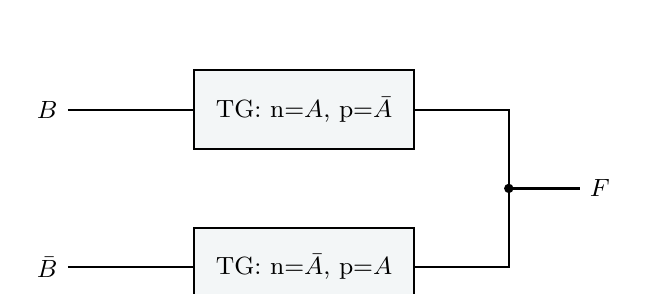
\begin{tikzpicture}[x=1cm,y=1cm,line width=.8pt,font=\small]
 \node[draw,minimum width=28mm,minimum height=10mm,fill=accent!5] (t1) at (0,0) {TG: n=$A$, p=$\bar A$};
 \node[draw,minimum width=28mm,minimum height=10mm,fill=accent!5] (t0) at (0,-2) {TG: n=$\bar A$, p=$A$};
 \draw (-3,0) node[left] {$B$}--(t1.west);
 \draw (-3,-2) node[left] {$\bar B$}--(t0.west);
 \draw (t1.east)--(2.6,0)--(2.6,-2)--(t0.east);
 \draw (2.6,-1)--(3.5,-1) node[right] {$F$};
 \fill (2.6,-1) circle (1.7pt);
\end{tikzpicture}
\end{center}
每個 TG 仍是第 3 頁所畫的兩顆並聯 MOS。兩個 TG 共 4T，加上產生
$\bar A,\bar B$ 的兩個 inverter 共 4T，合計 8T。$A=1$ 時只有上支導通，
$A=0$ 時只有下支導通，互斥選擇使 $B$ 與 $\bar B$ 不會直接短接。
主要答案仍採前頁 static CMOS，因為它明確展現 PUN/PDN 的互補結構。

\section*{參考答案比對、採用理由與來源}
原始題目：\texttt{homework1.pdf}，EE3032 Introduction to VLSI Design,
Jin-Fu Li, Fall 2024，共 1 頁。以下參考是使用者原始資料夾中的既有手寫檔案，
作者與授權均未標示；本解答沒有將其手寫內容當成自己的原創。
\begin{itemize}
 \item \textbf{參考 A：}\texttt{VLSI HW1 第三題(2)電路畫錯.pdf}，4 頁，
 第 1 頁是封面。已讀第 2--4 頁的所有解題內容。
 \item \textbf{參考 B：}\texttt{VLSI HW1.pdf}，3 頁。已讀全部解題內容。
\end{itemize}
\begin{tabular}{p{.10\linewidth}p{.38\linewidth}p{.44\linewidth}}\toprule
題目&比對結果&本解答採用方式\\\midrule
1(a)&兩份均保留未化簡的 10T 網路。A 的冗餘支路標成 $\bar z$，
不符合正相輸入限制；但因吸收律，該支路不影響輸出。&
依原題正確讀式，先吸收為 $\overline{x+y}$，採 4T NOR。\\
1(b)&兩份均畫出 12T 網路：PDN 為 $(x+y)(x+z)(y+z)$，邏輯正確。&
保留 minority 函數與互補原理，因式分解 PDN 為 $xy+z(x+y)$，改成 10T。\\
2&兩份的循環選擇接線符合原表；B 明畫反相控制，A 較簡略。&
保留有效接線，明畫 TG 的 n/p gate 與共用反相器，補齊 one-hot 條件與 40T 計數。\\
3&兩份均判為 XNOR。A 的 TG 互補控制橫線可辨，但上支 MOS 類型的符號不清；
B 的 static CMOS 結構正確。&
採獨立推導且與 B 一致的 static CMOS；另重畫明確標示 n/p gate 的完整 TG 版，
不以 A 的模糊符號斷言其接線錯誤。\\\bottomrule
\end{tabular}

\section*{可重現驗證}
\texttt{verify\_logic.py} 枚舉真值，同時依圖中的 MOS 端點建立導通圖：
題 1(a) 16 組、題 1(b) 8 組、題 2 有效規格 64 組、題 3 各版本 4 組。
它檢查 static CMOS 無浮接或電源直通，TG 輸出恰連到指定資料；
加上反相器與未指定控制碼的檢查，共 100 組案例。
這是理想二進位開關驗證，不是製程、延遲、動態切換或類比電壓的 HSPICE 模擬。
\end{document}
